\chapter{Background in continuum mechanics for soft-tissue modelling}
\label{chap2}
\begin{shortAbstract}
As seen in the previous chapter, realistic modelling of organ deformation is a challenging research field that opens the door to new clinical applications including: medical training and rehearsal systems, patient-specific planning of surgical procedures and per-operative guidance based on simulation. In all these cases the clinician needs fast updates of the deformation model to obtain a real-time display of the computed deformations. If for medical training devices the haptic feedback from touching organs merely needs to feel real, the accuracy of the information provided to the clinician in the cases of planning or per-operative guidance is crucial. Therefore, a substantial comprehension of the mechanics involved and a knowledge of the physical properties of anatomical structures are both mandatory in our quest to realistically model the deformation of organs. This chapter will start by introducing the main concepts of continuum mechanics that are fundamental to study the mechanical response of organs. It will then present mathematical models able to describe the different mechanical aspects of materials and briefly discuss the mechanical characterisation of tissues.
\end{shortAbstract}



\section{Introduction}
In our everyday life, matter appears smooth and continuous: from the wood used to build your desk to the water you drink. But this is just illusion. The concept that matter is composed of discrete units has been around for millennia. In fact, we know with certainty that our world is composed of microscopic atoms and molecules separated by empty space since the beginning of the twentieth century \citep{Lautrup05}. However, certain physical phenomena can be predicted with theories that pay no attention to the molecular structure of materials. Consider for instance the deformation of the horizontal board of a bookshelf under the weight of books. The bending of the shelf can be modelled without considering its molecular composition. The branch of physics in which materials are treated as continuous is known as \emph{continuum mechanics}. Continuum mechanics studies the response of materials to different loading conditions. In this theory, matter is assumed to exist as a continuum, meaning that the matter in the body is continuously distributed and fills the entire region of space it occupies \citep{Lai96}. This assumption is generally valid if the length scales of interest are large compared with the length scales of discrete molecular structure, but whether the approximation of continuum mechanics is actually justified in a given situation is merely a matter of experimental test. 

Modelling anatomical structures requires an understanding of the deformation and stresses caused by the different interactions that occur during medical procedures. A sufficient knowledge of continuum mechanics is therefore essential to follow the rest of this manuscript. Continuum mechanics can be divided into two main parts: general principles common to all media (analysis of deformation, strain and stress concepts) and constitutive equations defining idealised materials. This chapter will not only deal with those two aspects but will also discuss the different aspects of the mechanical behaviour that we find in anatomical structures. Note that this chapter will mostly follow the notation used by \cite{Bonnet97} and \cite{Reddy07}. The interested reader may refer to these books for more details.  
%This chapter will not only deal with those two aspects but will also introduce experiments carried out on organs in order to assess the physical parameters used in the mathematical models. 


\section{Description of motion} 	\label{chap2:descriptionMotion}
Let us consider a body $\textbf{\textit{B}}$ of known geometry in a three-dimensional Euclidian space $\field{R}^3$. For a given geometry and loading, $\textbf{\textit{B}}$ will undergo a set of macroscopic changes which is called \emph{deformation}. The region of space occupied by the body at a given time $t$ is termed a \emph{configuration}. A change in the configuration of a continuum body results in a displacement. The displacement of a body has two components: a rigid-body displacement and a deformation. A rigid-body displacement consists of a simultaneous translation and rotation of the body without changing its shape or size. \ON In constrast, a change in shape and\slash or size of the body from an initial configuration $\kappa_{0}$ to a new configuration $\kappa$ is called a deformation. This new configuration $\kappa$ may be designated by the \emph{current} or \emph{deformed configuration}. \OFF

Let us now consider a given particle of the body that we call $X$. What we will call particle in the following is in fact an infinitesimal volume of material. We denote the position it occupies in the initial configuration $\mathbf{X}$ and note its position in the deformed configuration $\mathbf{x}$, both expressed in the chosen frame of reference. The mapping $\chi$ defined as the following:
\begin{equation}
\label{chap2:mapping}
\chi : \textbf{\textit{B}}_{\kappa_{0}} \rightarrow \textbf{\textit{B}}_{\kappa}
\end{equation} 
is called the \emph{deforming mapping} of the body $\textbf{\textit{B}}$ from $\kappa_{0}$ to $\kappa$. When analysing the deformation of a continuous body, it is necessary to describe the evolution of configurations through time. Its mathematical description follows one of the two approaches: the material description or the spatial description. The material description is known as \emph{Lagrangian description} whereas the spatial description is called \emph{Eulerian description}. These two approaches are detailed next. 

	\subsection{Lagrangian description}	
In the Lagrangian description, the position and physical properties of the particles are referred to a reference configuration $\kappa_{R}$, often chosen to be the undeformed configuration $\kappa_{0}$. \ON Consequently, the current coordinates ($\mathbf{x} \in \kappa$) depend on the reference coordinates ($\mathbf{X} \in \kappa_{0}$): \OFF
\begin{equation}
\textbf{x} = \chi(\textbf{X}, t), \quad \chi(\textbf{X}, 0) = \textbf{X},
\end{equation}
\ON and a typical variable $\phi$ defined over the body is expressed in terms of the coordinates $\mathbf{X}$ and time $t$: \OFF
\begin{equation}
\label{chap2:phi}
\phi = \phi(\textbf{X}, t).
\end{equation}
\ON Let us consider a particule $X$ whose position in the reference configuration is $\mathbf{X}$. From \eqref{chap2:phi}, we note that the value of $\phi$ associated with this fixed particle $X$ changes over time. Hence, \OFF the Lagrangian description focuses its attention on the particles of the continuous body and it is usually used in solid mechanics.
	
	\subsection{Eulerian description}
\ON In constrast, the Eulerian description is interested in changes at fixed locations. This time, the motion and $\phi$ are described with respect to the current position ($\mathbf{x} \in \kappa$): \OFF
\begin{equation}
\phi = \phi(\textbf{x}, t), \quad \textbf{X} = \textbf{X}(\textbf{x}, t).
\end{equation}
For a fixed value of $\mathbf{x} \in \kappa$, $\phi(\mathbf{x},t)$ gives the value of $\phi$ associated with the particle occupying the position $\textbf{x} \in \kappa$, which may very well be a different particle for each new time $ t $. Because a change in time $t$ implies that a different value $\phi$ is observed at the same spatial location $\mathbf{x} \in \kappa$, now probably occupied by a different particle, the Eulerian description is focused on a spatial position. This approach is convenient for the study of fluid flow where the kinematic property of greatest interest is the rate at which change is taking place rather than the shape of the body of fluid at a reference time \citep{Spencer80}. Because we are only interested in the study of solid bodies, the Lagrangian description will be used in the rest of the text. 
	
	\subsection{Displacement field}
The displacement $ \mathbf{u} $ of a particle $X$ is called \emph{displacement vector} and its expression in the Lagrangian description is given by the following:
\begin{equation}
\mathbf{u}(\textbf{X}, t) = \mathbf{x}(\mathbf{X}, t) - \mathbf{X}.
\end{equation}
A \emph{displacement field} is a vector field of all displacement vectors for all particles in the body. \ON Thus, the deformed configuration $\kappa$ may be obtained from the undeformed configuration $\kappa_{0}$ by merely adding the displacement field: \OFF $\kappa_{0}$: $\chi(\mathbf{X}, t) = \mathbf{X} + \mathbf{u}(\mathbf{X})$. 
	
\section{Analysis of deformation}

	\subsection{Deformation gradient tensor}
The displacement field tells us how a \ON particule \OFF displaces from the reference to the deformed configuration. \ON More interestingly, we would like to know how a material line would deform (stretch and rotation) within this displacement field. \OFF Since the length of a material line $d\mathbf{X}$ can change when going to the deformed configuration as well as its orientation, we can say that $d\mathbf{X}$ deforms into $d\mathbf{x}$. \ON We now seek the relation existing between $d\mathbf{x}$ in the deformed configuration and $d\mathbf{X}$ of the reference configuration. \OFF

Consider two particles $P_{1}$ and $P_{2}$ in a continuous body separated by an infinitesimal distance $d\mathbf{X}$:
\begin{equation}
\label{chap2:dX}
d\mathbf{X} = \mathbf{X}_{P_{2}} - \mathbf{X}_{P_{1}}.
\end{equation}
After deformation, the two particles have deformed to their current positions given by the mapping $\chi$~\eqref{chap2:mapping} as:
\begin{equation}
\mathbf{x}_{P_1} = \chi(\mathbf{X}_{P_{1}}, t) \quad \mbox{and} \quad \mathbf{x}_{P_2} = \chi(\mathbf{X}_{P_{2}}, t).
\end{equation}
Using \eqref{chap2:dX} the distance $d\textbf{x}$ between $P_{1}$ and $P_{2}$ can then be expressed as:
\begin{equation}
d\mathbf{x} = \mathbf{x}_{P_{2}} - \mathbf{x}_{P_{1}} = \chi(\mathbf{X}_{P_{1}} + d\mathbf{X}, t) - \chi(\mathbf{X}_{P_{1}}, t).
\end{equation}
The \emph{deformation gradient} $\textbf{F}$ can be defined as:
\begin{equation}
\mathbf{F} = \pd{\chi}{\mathbf{X}}
\end{equation}
and the vector $d\textbf{x}$ can then be obtained in terms of $d\mathbf{X}$ as:
\begin{equation}
\label{chap2:dxdX}
d\textbf{x} = \textbf{F} \, d\textbf{X}.
\end{equation}
Note that $\textbf{F}$ transforms vectors from the reference configuration into vectors in the current configuration and is therefore a second-order tensor.

Knowing that $\chi(\mathbf{X}, t)$ is of course $\mathbf{x}$, the deformation gradient may also be written as:
\begin{equation}
\label{chap2:gradient}
\mathbf{F} = \pd{\mathbf{x}}{\mathbf{X}} = \nabla_{0} \mathbf{x} = \nabla_{0} \mathbf{u} + \mathbf{I},
\end{equation}
where $\nabla_{0}$ is the gradient operator with respect to $\mathbf{X}$ and $\mathbf{u}$ the displacement vector. In indicial notation in a Cartesian coordinate system, \eqref{chap2:gradient} can be explicited as:
\begin{equation}
[F] = 
	\begin{bmatrix}
		\pd{\mathbf{x}_{1}}{\mathbf{X}_{1}} & \pd{\mathbf{x}_{1}}{\mathbf{X}_{2}} & \pd{\mathbf{x}_{1}}{\mathbf{X}_{3}} \\\\
		\pd{\mathbf{x}_{2}}{\mathbf{X}_{1}} & \pd{\mathbf{x}_{2}}{\mathbf{X}_{2}} & \pd{\mathbf{x}_{2}}{\mathbf{X}_{3}} \\\\
		\pd{\mathbf{x}_{3}}{\mathbf{X}_{1}} & \pd{\mathbf{x}_{3}}{\mathbf{X}_{2}} & \pd{\mathbf{x}_{3}}{\mathbf{X}_{3}}
	\end{bmatrix}
	.
\end{equation}


	\subsection{Change of volume}
At this point, we have seen how a deformation can affect a vector. We will now look into its effect on volumes. Our motivation comes from the need to write global equilibrium statements that involve integrals over volumes. \ON Let us consider a volume in the reference configuration formed by \OFF three non-coplanar line elements $d\mathbf{X}^{(1)}$, $d\mathbf{X}^{(2)}$ and $d\mathbf{X}^{(3)}$ as can be seen on \fig{chap2:fig-changeVolume}.
% 
\begin{figure}[h]
\begin{center}
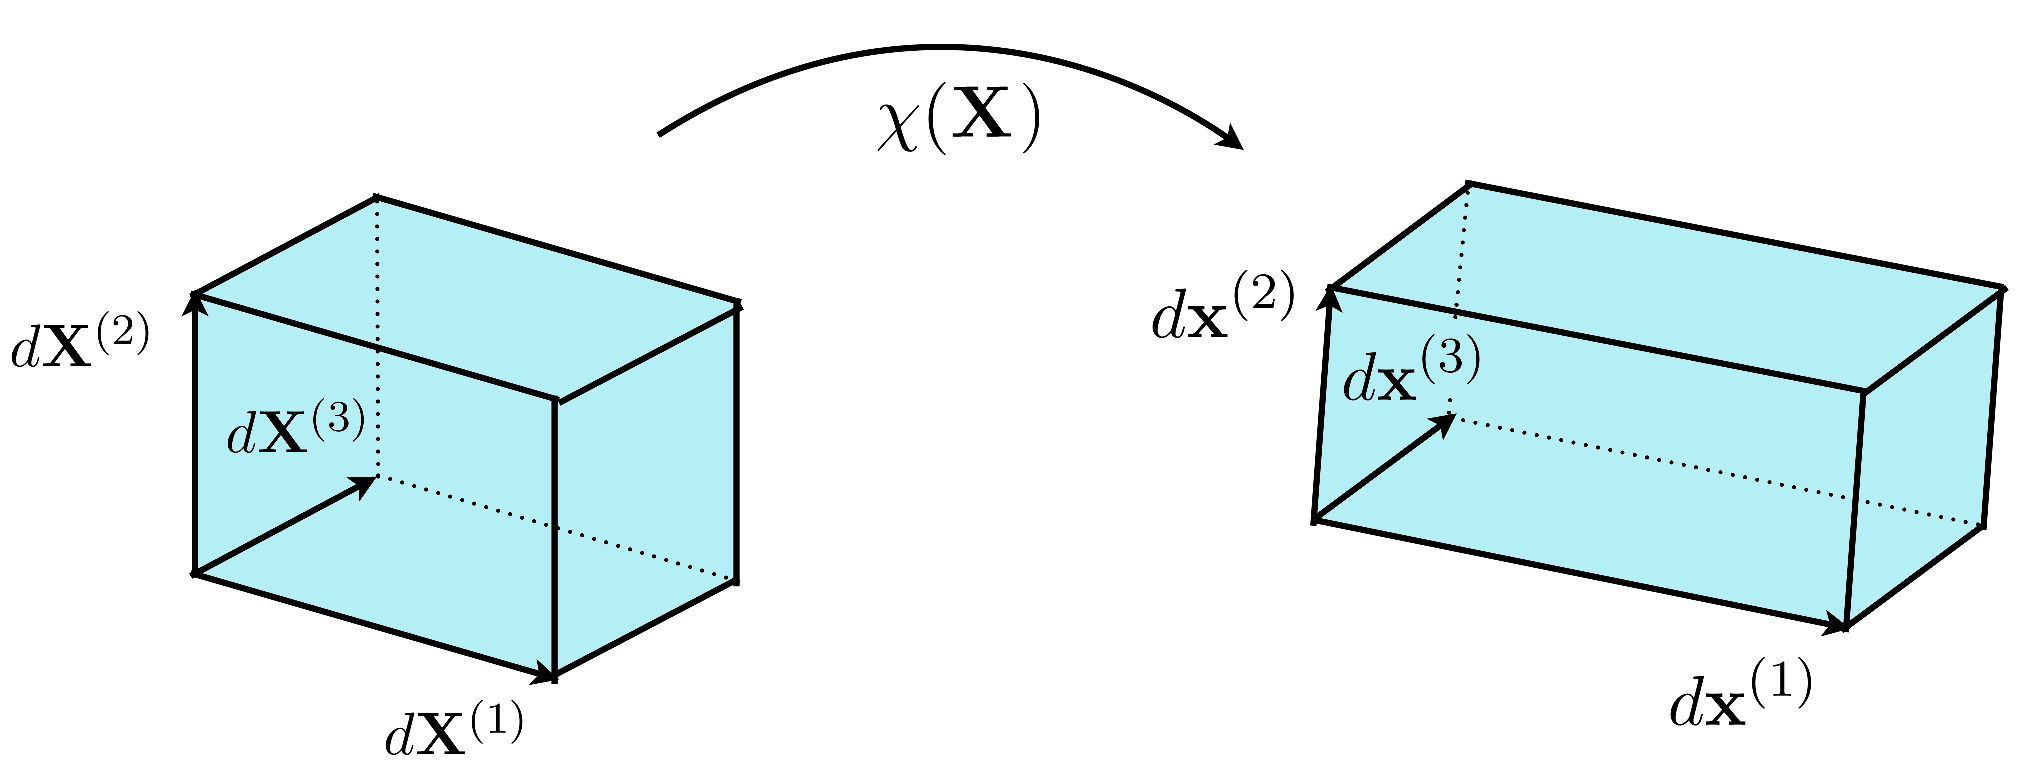
\includegraphics[width=12cm]{chapter2/changeVolume.pdf}
\end{center}
\caption{Transformation of a volume element under a deformation mapping.}
\label{chap2:fig-changeVolume}
\end{figure}
%

The three vectors after deformation $d\mathbf{x}^{(1)}$, $d\mathbf{x}^{(2)}$ and $d\mathbf{x}^{(3)}$ can be obtained with:
\begin{equation}
\label{chap2:dxdX}
d\mathbf{x}^{(i)} = \mathbf{F} \, d\mathbf{X}^{(i)}, \quad i = 1, 2, 3.
\end{equation}
The volume of the parallelepiped that we will note $dV$  can be calculated using the triple product between the three vectors:
\begin{align}
dV &= d\mathbf{X}^{(1)} \cdot d\mathbf{X}^{(2)} \times d\mathbf{X}^{(3)} = (\mathbf{\hat{N}}_{1} \cdot \mathbf{\hat{N}}_{2} \times \mathbf{\hat{N}}_{3}) \, dX^{(1)} dX^{(2)} dX^{(3)} \notag \\
&= dX^{(1)} dX^{(2)} dX^{(3)}, \label{chap2:dV}
\end{align}
where $\mathbf{\hat{N}}_{i}$ \ON is \OFF the unit vector along $d\mathbf{X}^{i}$. \ON Similarly, we can compute the \OFF corresponding volume in the deformed configuration by:
\begin{align}
dv &= d\mathbf{x}^{(1)} \cdot d\mathbf{x}^{(2)} \times d\mathbf{x}^{(3)} \notag \\
&=  (\mathbf{F} \cdot \mathbf{\hat{N}}_{1}) \cdot (\mathbf{F} \cdot \mathbf{\hat{N}}_{2}) \times (\mathbf{F} \cdot \mathbf{\hat{N}}_{3}) \,  dX^{(1)} dX^{(2)} dX^{(3)} \quad \text{by \eqref{chap2:dxdX}} \notag \\
&= \det \mathbf{F} \, dX^{(1)} dX^{(2)} dX^{(3)}. \label{chap2:dv}
\end{align}
The determinant of $\mathbf{F}$ is called the \emph{Jacobian} and it is denoted by $J = \det \mathbf{F}$. \ON Therefore, the relation between the deformed volume $ dv $ and the undeformed volume $ dV $ may be written as: \OFF
\begin{equation}
\label{chap2:dvdV}
dv = J dV.
\end{equation}
\ON It is worth noting that the Jacobian \OFF  J has the physical meaning of being the local ratio of current to reference volume of a material volume element.


	\subsection{Change of surface}
For similar reasons, let us find the relation between an element of area in the reference configuration $d\mathbf{A}$ which becomes $d\mathbf{a}$ in the deformed configuration. Considering an arbitrary material line $d\mathbf{L}$ in the reference configuration and noting $d\mathbf{l}$ the same line after deformation, the reference and current volumes are given respectively by:
\begin{align}
d\mathbf{V} &= d\mathbf{L} \cdot d\mathbf{A} \\
\mbox{and } \quad d\mathbf{v} &= d\mathbf{l} \cdot d\mathbf{a}.
\end{align}
Using \eqref{chap2:dvdV} which relates the reference and deformed volumes and recalling that $d\mathbf{l} = \mathbf{F} \, d\mathbf{L}$, we have:
\begin{equation}
J \, d\mathbf{L} \cdot d\mathbf{A} = (\mathbf{F} \, d\mathbf{L}) \cdot d\mathbf{a}.
\end{equation}
\ON Since \OFF this expression is valid for any vector $d\mathbf{L}$ and by using the property $\mathbf{a} \cdot \mathbf{b} = \mathbf{a} ^{T} \mathbf{b}$, \ON the sought relation between an element of area in the reference configuration $d\mathbf{A}$ and its corresponding area $d\mathbf{a}$ in the deformed configuration may be expressed as: \OFF
\begin{equation}
\label{chap2:dadA}
d\mathbf{a} = J \, \mathbf{F}^{-T} \, d\mathbf{A}.
\end{equation}
% 
%\begin{figure}[h]
%\begin{center}
%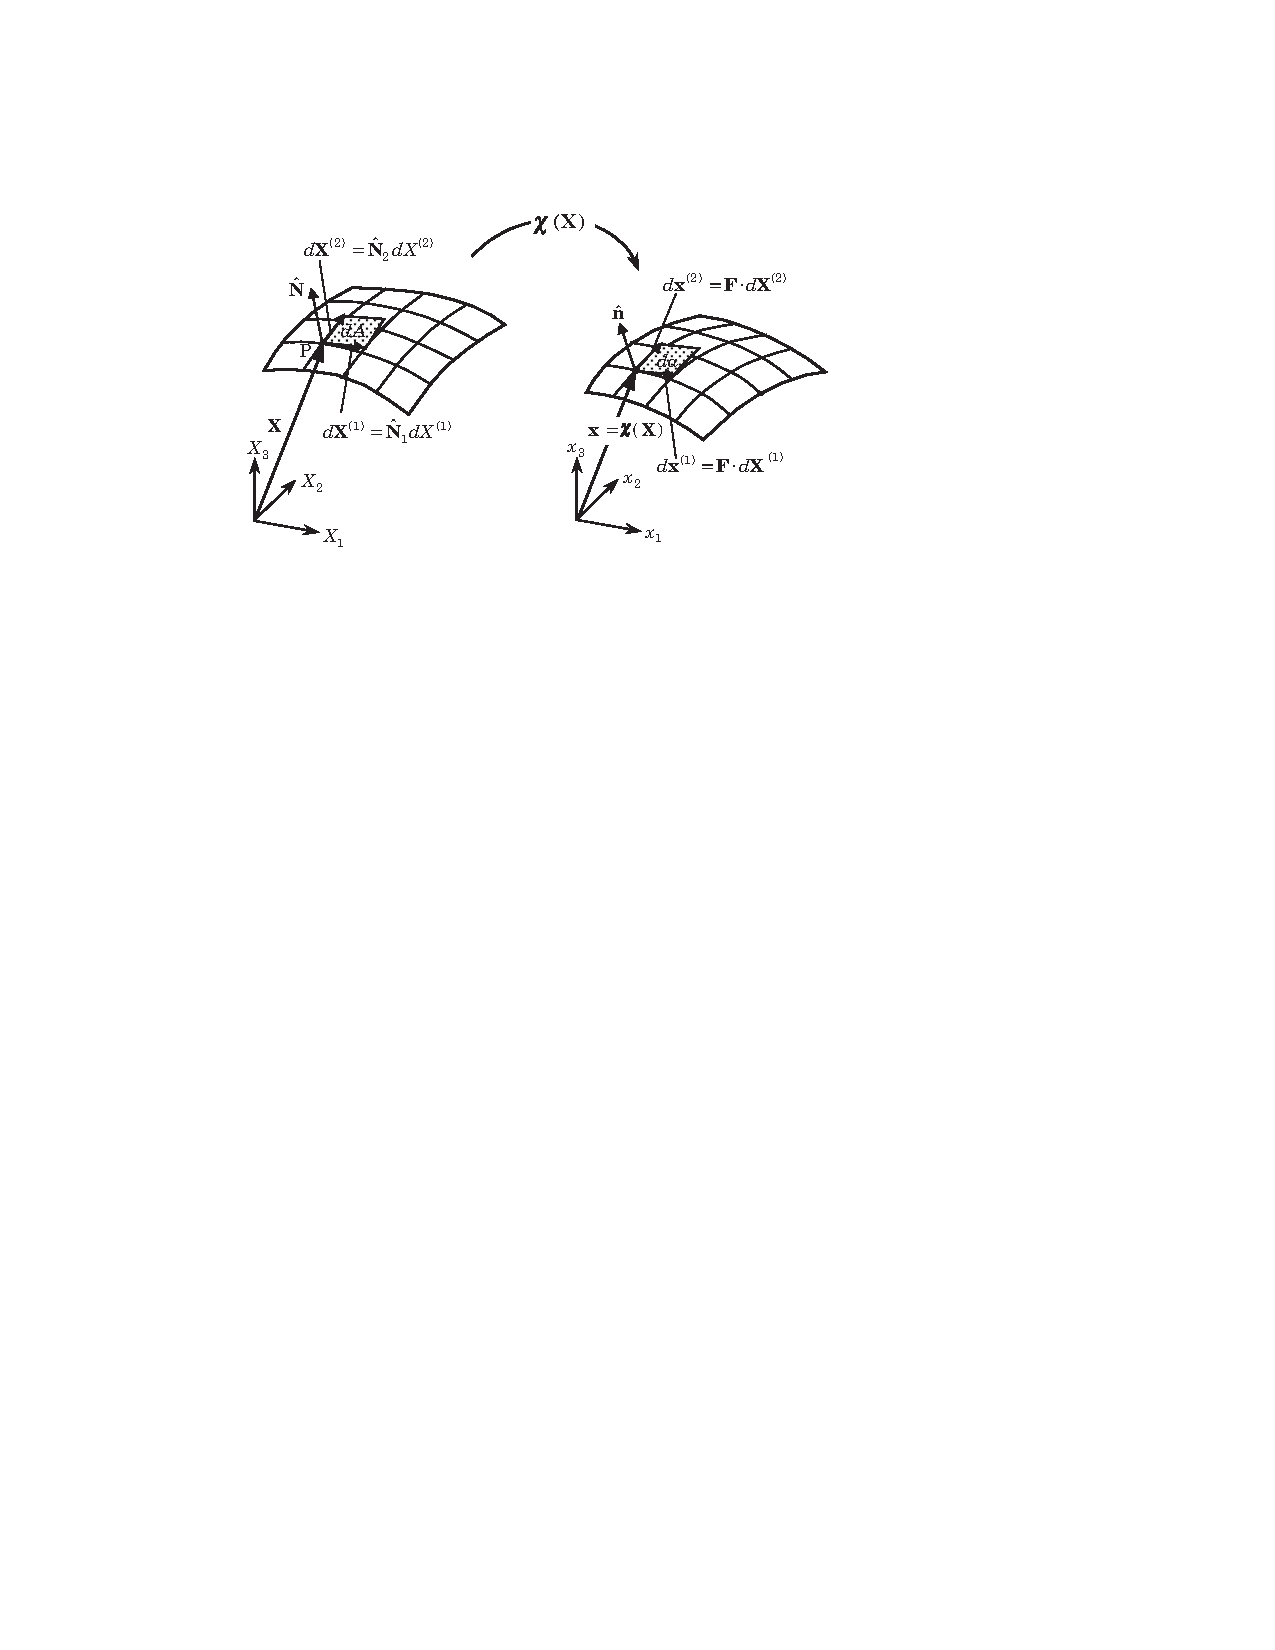
\includegraphics[width=13cm]{chapter2/changeSurface.pdf}
%\end{center}
%\caption{Transformation of a surface element under a deformation mapping. \TODO{CHANGE TO A BETTER FIGURE.}}
%\label{chap2:fig-changeSurface}
%\end{figure}
			
	\subsection{Volumetric and isochoric components}
We recall that the Jacobian $J$ has the physical meaning of being the local ratio of current to reference volume of a material volume element. Therefore, if $J = 1$ the volume does not change locally during the deformation and the latter is qualified as \emph{isochoric} at this given particle $P$. If $J = 1$ everywhere in the body, the deformation of the body is isochoric. 

When dealing with incompressible and nearly incompressible materials it is necessary to separate the volumetric from the isochoric components of the deformation. Such a separation must ensure that the isochoric component $\mathbf{\hat{F}}$ does not imply any change in volume. This condition can be achieved by choosing $\mathbf{\hat{F}}$ as:
\begin{equation}
\mathbf{\hat{F}} = J^{-1/3} \mathbf{F}.
\end{equation}
Indeed,
\begin{align}
\det \mathbf{\hat{F}} &= \det (J^{-1/3} \mathbf{F}) \notag \\
&= (J^{-1/3})^3 \det \mathbf{F} \notag \\
&= J^{-1} J \notag \\
&= 1.
\end{align}
The deformation gradient $\mathbf{F}$ can now be expressed in terms of the volumetric and isochoric component $J$ and $\mathbf{\hat{F}}$ as:
\begin{equation}
\mathbf{F} = J^{1/3} \mathbf{\hat{F}}.
\end{equation}
			
			
\section{Strain measures}	\label{chap2:strainMeasures}
The length of a material curve from the reference configuration can change when displaced to a curve in the deformed configuration. If all the curves do not change length, it is said that a rigid body displacement occurred. The concept of strain is used to evaluate how much a given displacement differs locally from a rigid body displacement \citep{Lubliner06}. Therefore, although we know how to transform vectors from the reference configuration into vectors in the current configuration using the deformation gradient, it is more useful to find a measure of the change in length of $d\mathbf{X}$. Many measures of strains can be defined and the most common ones will now be introduced. 

	\subsection{Cauchy-Green deformation tensors}
Let us consider two particles $P_{1}$ and $P_{2}$ in the neighbourhood of each other, separated by $d\mathbf{X}$ in the reference configuration. In the deformed configuration $P_{1}$ and $P_{2}$ occupy the positions $\tilde{P}_{1}$ and $\tilde{P}_{2}$ and they are separated by $d\mathbf{x}$. We are interested in the change of distance between the two points $P_{1}$ and $P_{2}$ as the body deforms. 

The squared distances between $P_{1}$ and $P_{2}$ and $\tilde{P}_{1}$ and $\tilde{P}_{2}$ are respectively given by:
\begin{align}
(dS)^2 &= d\mathbf{X} \cdot d\mathbf{X} \label{chap2:dS} \\
(ds)^2 &= d\mathbf{x} \cdot d\mathbf{x} = (\mathbf{F} \, d\mathbf{X}) \cdot (\mathbf{F} \, d\mathbf{X}) \notag \\
&= (\mathbf{F} \, d\mathbf{X})^T (\mathbf{F} \, d\mathbf{X}) = (d\mathbf{X}^T \, \mathbf{F}^T) (\mathbf{F} \, d\mathbf{X}) = d\mathbf{X}^T (\mathbf{F}^T \mathbf{F} \, d\mathbf{X}) \notag \\
&= d\mathbf{X} \cdot (\mathbf{F}^T \mathbf{F} \, d\mathbf{X}).
\end{align}
using the property that the dot product between two vectors $a$ and $b$ can also be expressed as the simple product between the transpose of $a$ and $b$ ($a \cdot b = a^T b$). We define the \emph{right Cauchy-Green deformation tensor} $\mathbf{C}$ as:
\begin{equation}
\mathbf{C} = \mathbf{F}^T \mathbf{F}.
\end{equation}
Thus, the change of distance between the two points $P_{1}$ and $P_{2}$ after deformation of the continuous body may be written as:
\begin{equation}
\label{chap2:ds}
(ds)^2 = d\mathbf{X} \cdot (\mathbf{C} \, d\mathbf{X}).
\end{equation}
By definition, $\mathbf{C}$ is a symmetric second-order tensor. The transpose of $\mathbf{C}$ is denoted $\mathbf{B}$ and is called the \emph{left Cauchy-Green deformation tensor}:
\begin{equation}
\mathbf{B} = \mathbf{F} \mathbf{F}^T.
\end{equation}

	
	\subsection{Green-Lagrange strain tensor}
Using \eqref{chap2:dS} and \eqref{chap2:ds}, \ON the difference in the squared lengths between the reference and the current configuration may be evaluated as: \OFF 
\begin{align}
(ds)^2 - (dS)^2 &= d\mathbf{X} \cdot (\mathbf{C} \, d\mathbf{X}) - d\mathbf{X} \cdot d\mathbf{X} \notag \\
&= d\mathbf{X} \cdot  (\mathbf{C} - \mathbf{I}) \, d\mathbf{X}.
\end{align}
Let us define the \emph{Green-Lagrange strain tensor} $\mathbf{E}$ as:
\begin{equation}
\mathbf{E} = \frac{1}{2}	 (\mathbf{C} - \mathbf{I})
\end{equation}
so we can write:
\begin{equation}
(ds)^2 - (dS)^2 = 2 \, d\mathbf{X} \cdot \mathbf{E} \, d\mathbf{X}.
\end{equation}
By definition, the Green-Lagrange strain tensor is a symmetric second-order tensor. \ON Moreover, we observe that \OFF the change in squared lengths is zero if and only if \ON the Green-Lagrange strain tensor \OFF $\mathbf{E} = \mathbf{0}$. Using \eqref{chap2:gradient}, the Green strain tensor may be expanded as the following:
\begin{align}
\mathbf{E} &= \frac{1}{2} (\mathbf{F}^T \mathbf{F} - \mathbf{I}) \notag \\
&= \frac{1}{2} \left[ (\nabla_{0} \mathbf{u} + \mathbf{I})^T (\nabla_{0} \mathbf{u} + \mathbf{I}) - \mathbf{I} \right] \notag \\
&= \frac{1}{2} \left[ (\nabla_{0} \mathbf{u})^T  + \nabla_{0} \mathbf{u}+ (\nabla_{0} \mathbf{u})^T(\nabla_{0} \mathbf{u}) \right]. \label{chap2:GreenTensor}
\end{align}

The Green strain tensor can be expressed in terms of its components in any coordinate system. In particular, in the Cartesian coordinate system $(X_1, X_2, X_3)$ the components $E_{ij}$ of $\mathbf{E}$ are the following:
\begin{equation}
E_{i,j} = \frac{1}{2} \left( \pd{u_i}{Xj} + \pd{u_j}{Xi} + \pd{u_k}{Xi} \pd{u_k}{Xj} \right), \quad i = 1, 2, 3.
\end{equation}
The components $E_{11}$, $E_{22}$ and $E_{33}$ are called \emph{normal strains} and it can be shown that they are in fact the ratio of the change in length to the original length along each of the three unit vectors. The components $E_{12}$, $E_{23}$ and $E_{13}$ are called \emph{shear strains} and they can be interpreted as a measure of the change in angle between line elements that were perpendicular to each other in the undeformed configuration. 

	\subsection{Cauchy and Euler tensor}
The change in the squared lengths during the body deformation can also be expressed relative to the current length. The length $dS$ can be written in terms of $d\mathbf{x}$ as:
\begin{equation}
(dS)^2 = d\mathbf{X} \cdot d\mathbf{X} = d\mathbf{x} \cdot (\mathbf{F}^{-T} \mathbf{F}^{-1}) d\mathbf{x} = d\mathbf{x} \cdot \mathbf{\tilde{B}} d\mathbf{x}
\end{equation}
where $\mathbf{\tilde{B}} = \mathbf{F}^{-T} \mathbf{F}^{-1}$ is called the \emph{Cauchy strain tensor}. $\mathbf{\tilde{B}}$ is in fact the inverse of the left Cauchy-Green tensor $\mathbf{B}$ introduced previously. 

In a similar way we defined the Green strain tensor, we can write the change in the squared lengths but relative to the current length:
\begin{equation}
(ds)^2 - (dS)^2 = 2 \, d\mathbf{x} \cdot \mathbf{e} \, d\mathbf{x}.
\end{equation}
where $\mathbf{e}$ is called \emph{Almansi-Hamel strain tensor} or simply \emph{Euler strain tensor}. 

	
	\subsection{Principal strains and invariants}	\label{chap2:strainInvariants}
The components $\varepsilon_{ij}$ of the strain tensor depend on the coordinate system at the point under consideration. However, the strain tensor itself is a physical quantity and as such, it is independent of the coordinate system chosen to represent it. Certain operations on strain tensors give the same result independently of the coordinate system chosen to represent the components of strain. As an example, a vector is a simple tensor of rank one. In three dimensions, it has three components. The value of these components will depend on the coordinate system chosen to represent the vector, but the length of the vector is a physical quantity (a scalar) and is independent of the coordinate system chosen to represent the vector. Similarly, every second rank tensor (such as the strain tensors) has three independent invariant quantities associated with it. One set of such \emph{invariants} are the principal strains of the strain tensor, which are just the eigenvalues of the strain tensor. Because they are independent of any coordinate system, they are very convenient to define strain energy density functions (see section \ref{chap2:non-linear}). The most commonly used invariants are:
\begin{align}
I_1 &= tr(\varepsilon) \notag \\
I_2 &= \frac{1}{2} \left\lbrace tr(\varepsilon^{2}) - \left[tr(\varepsilon)\right]^{2} \right\rbrace \\
I_3 &= det(\varepsilon). \notag
\end{align}

It can be shown that in the coordinate system $(\mathbf{p}_1, \mathbf{p}_2, \mathbf{p}_3)$ formed by the three eigenvectors, the expression of the strain tensor is:
\begin{equation}
\boldsymbol \varepsilon =
	\begin{bmatrix}
	\varepsilon_1 &          0           &           0           \\
	         0           & \varepsilon_2 &           0           \\
	         0           &           0           & \varepsilon_3
	\end{bmatrix}	
	.
\end{equation}
Since there are no shear strain components in this particular coordinate system, the principal strains represent the maximum and minimum stretches of an elemental volume. Because of the obvious simplicity of the strain tensor's expression, this coordinate system is often used in mechanics to derive and solve equations.

		
	\subsection{Infinitesimal strain tensor} \label{chap2:infinitesimalStrainTensor}
In some cases, it is possible to simplify the expression of the Green strain tensor defined in \eqref{chap2:GreenTensor}. Indeed, when the displacement gradients are small (that is, $|\nabla \mathbf{u}| \ll 1$) we can neglect the non-linear terms in the definition. In the case of infinitesimal strains, the Green-Lagrange strain tensor and the Eulerian strain tensor are approximately the same and can be approximated by the infinitesimal strain tensor denoted $\boldsymbol \varepsilon$ and is given by:
\begin{equation}
\boldsymbol \varepsilon = \frac{1}{2} \left[ \nabla \mathbf{u} + (\nabla \mathbf{u})^T \right].
\end{equation}
Its Cartesian components $\varepsilon_{ij}$ are the following:
\begin{equation}
\varepsilon_{ij} = \frac{1}{2} (\pd{u_i}{X_j} + \pd{u_j}{X_i}).
\end{equation}

The strain quantities defined in the previous sections are non-linear expressions in terms of the mapping $\chi$ and will lead to non-linear governing equations. In solid mechanics, whenever the hypothesis is acceptable, it is common practice to assume that the displacements are small and the infinitesimal strain tensor is then used as a measure of the deformation. 

\section{Stress}
Stress is a measure of the intensity of the internal forces acting between particles of a deformable body across imaginary internal surfaces. These internal forces are produced between the particles in the body as a reaction to external forces applied on the body. The SI unit for stress is pascal (symbol $Pa$), which is equivalent to one newton (force) per square metre (unit area). As with strain, stress can be measured per unit of deformed area (section \ref{chap2:CauchyStress}) or undeformed area (sections \ref{chap2:PiolaStress1} and \ref{chap2:PiolaStress2}). In general, the stress is not uniformly distributed over the cross section of a material body, and consequently the stress at a point on a given area is different from the average stress over this entire area. Therefore, it is necessary to define the stress not over a given area but at a specific point in the body. \ON The stress at a point in a three-dimensional continuum is fully defined by \OFF nine quantities, three per plane, on three mutually perpendicular planes at the point. \ON The \emph{stress tensor} is defined as the second-order tensor which components are these nine quantities. \OFF 

	\subsection{Cauchy stress}\label{chap2:CauchyStress}
The Euler-Cauchy's stress principle states that on any surface (real or imaginary) that divides the body, the action of one part of the body on the other is equivalent to the system of distributed forces and couples on the surface dividing the body \citep{Truesdell60}. With that consideration in mind, let us consider a plane $S$ that passes through an arbitrary internal point $P$ which has a unit normal vector $\mathbf{n}$. This plane separates the body into two regions and we are interested in the forces applied by one region onto the other. First we will introduce the true stress, defined as the stress in the deformed configuration $\chi$ measured per unit area of the deformed configuration. The force $\Delta\mathbf{f}(\mathbf{n})$ acting on a small element of area $\Delta a$ in a continuous medium depends not only on the size of the area but also depends on the orientation of this area $\mathbf{n}$. The \emph{Cauchy stress vector} at $P$ on $S$ can be defined as:
\begin{equation}
\mathbf{t}(\mathbf{n}) = \lim_{\Delta a \to 0} \frac{\Delta \mathbf{f}(\mathbf{n})}{\Delta a}.
\end{equation}
This equation means that the stress vector depends on its location in the body and the orientation of the plane on which it is acting. In general, the stress vector is not perpendicular to that plane and it can be separated into two components: one component normal to the plane called \emph{normal stress} and one component tangent to the plane named \emph{shear stress}. Since $\mathbf{t}$ depends on $\mathbf{n}$ but is not in the direction of $\mathbf{n}$, it may be interesting to look into the relationship between $\mathbf{t}$ and $\mathbf{n}$. 

\ON In the following we make use of a Cartesian coordinate system and we consider an infinitesimal tetrahedron as shown on \fig{chap2:fig-CauchyStress}. \OFF
%
\begin{figure}[h]
\begin{center}
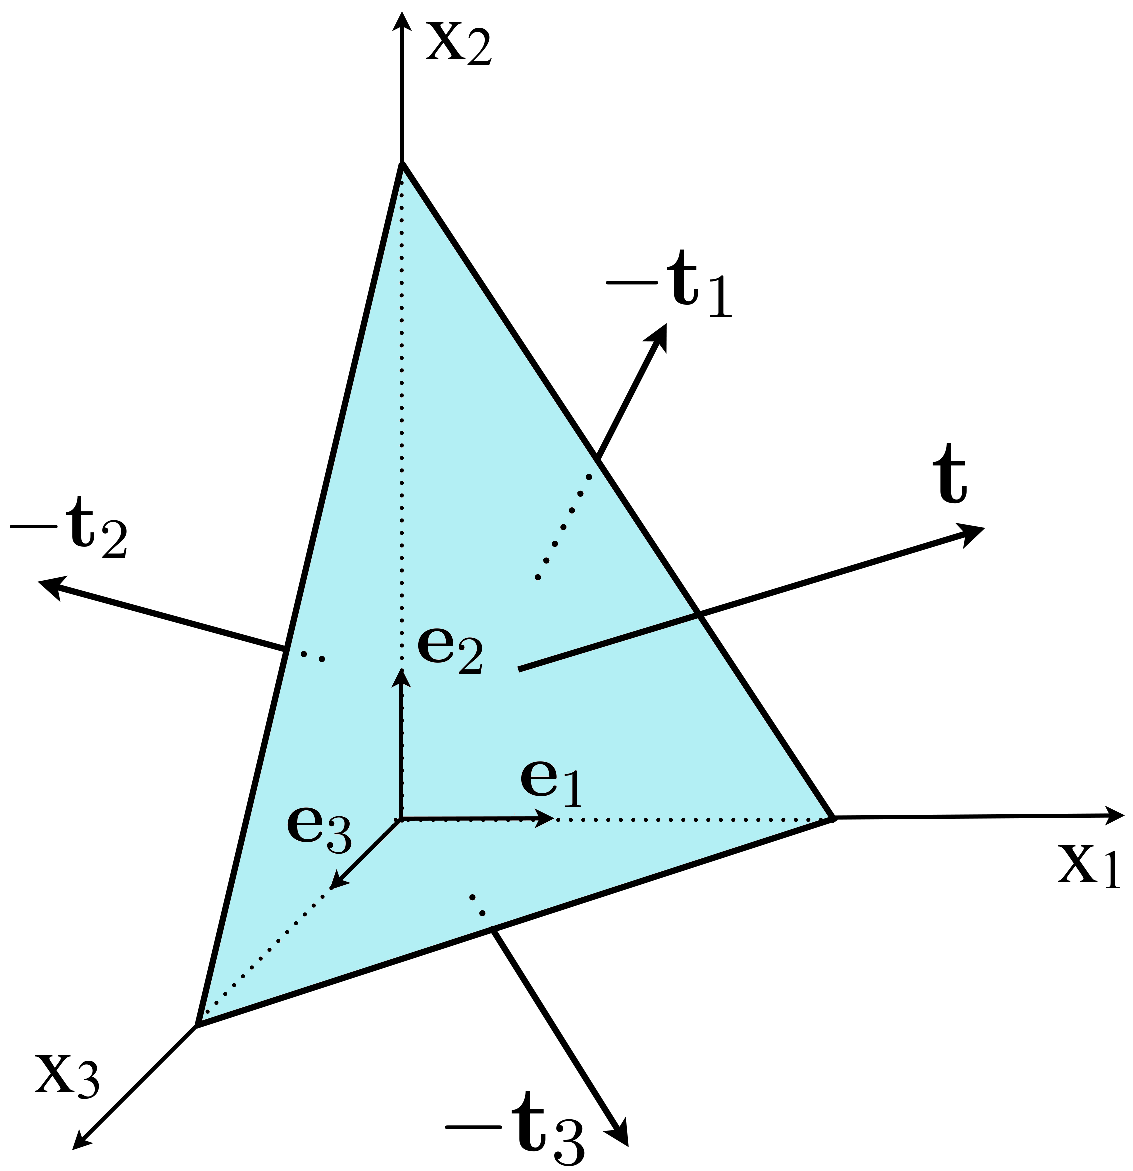
\includegraphics[width=6cm]{chapter2/CauchyStress.pdf}
\end{center}
\caption{Tetrahedral element in Cartesian coordinates.}
\label{chap2:fig-CauchyStress}
\end{figure}
%
We note $-\mathbf{t}_1$, $-\mathbf{t}_2$, $-\mathbf{t}_3$ and $\mathbf{t}$ the stress vectors in the outwards directions on the faces of the tetrahedron whose areas are respectively $\Delta a_1$, $\Delta a_2$, $\Delta a_3$ and $\Delta a$. For the mass $m$ inside the tetrahedron, we have by Newton's second law:
\begin{equation}
\label{chap2:Newton}
\sum \mathbf{F} = \mathbf{t} \Delta a - \mathbf{t}_1 \Delta a_1 - \mathbf{t}_2 \Delta a_2 - \mathbf{t}_3 \Delta a_3 + \Delta v \mathbf{f} = m \mathbf{a},
\end{equation}
where $\mathbf{f}$ is the force per unit volume acting on the body, $\Delta v$ the volume of the tetrahedron and $\mathbf{a}$ the acceleration.
The areas $\Delta a_1$, $\Delta a_2$ and $\Delta a_3$ being the projections of $\Delta a$, they are related to $\Delta a$ in the Cartesian coordinate system $(\mathbf{e}_1, \mathbf{e}_2, \mathbf{e}_3)$ by:
\begin{equation}
\label{chap2:DeltaAi}
\Delta a_i = (\mathbf{n} \cdot \mathbf{e}_i) \Delta a, \quad i=1, 2, 3.
\end{equation}
Dividing \eqref{chap2:Newton} by $\Delta a$, using \eqref{chap2:DeltaAi} and noting that $\Delta v \slash \Delta a \rightarrow 0$ when the tetrahedron shrinks to a point yields:
\begin{align}
\mathbf{t} &= (\mathbf{n} \cdot \mathbf{e}_1) \mathbf{t}_1 + (\mathbf{n} \cdot \mathbf{e}_2) \mathbf{t}_2 + (\mathbf{n} \cdot \mathbf{e}_3) \mathbf{t}_3 \notag \\
&= \mathbf{n} \cdot (\mathbf{e}_1 \mathbf{t}_1 + \mathbf{e}_2 \mathbf{t}_2 + \mathbf{e}_3 \mathbf{t}_3).
\end{align}

We define the \emph{Cauchy stress tensor} $\sigma = \mathbf{e}_1 \mathbf{t}_1 + \mathbf{e}_2 \mathbf{t}_2 + \mathbf{e}_3 \mathbf{t}_3$ and we have:
\begin{equation}
\label{chap2:CauchyFormula}
\mathbf{t}(\mathbf{n}) = \mathbf{n} \cdot \sigma .
\end{equation}
The stress vector $\mathbf{t}$ represents the vectorial stress on a plane whose normal is $\mathbf{n}$. As we demonstrated, the stress tensor is a property of the medium that is independent of $\mathbf{n}$. It represents the current force per unit of deformed area: $d\mathbf{f} = \mathbf{t} da = \sigma \cdot d\mathbf{a}$. 

The matrix form of \eqref{chap2:CauchyFormula} in a Cartesian coordinate system is given by:
\begin{equation}
	\begin{bmatrix}
		t_1 \\
		t_2 \\
		t_3
	\end{bmatrix}
= 
	\begin{bmatrix}
		\sigma_{11} & \sigma_{21} & \sigma_{31} \\
		\sigma_{12} & \sigma_{22} & \sigma_{32} \\
		\sigma_{13} & \sigma_{23} & \sigma_{33} \\
	\end{bmatrix}
	\begin{bmatrix}
		n_1 \\
		n_2 \\
		n_3
	\end{bmatrix}
	.
\end{equation}

The Cauchy stress tensor is used for stress analysis of material bodies experiencing small deformations. This stress is basically defined as force/(unit deformed area). The strain measure that is appropriate to use with the Cauchy stress tensor is \ON therefore \OFF the infinitesimal strain tensor (see section~\ref{chap2:infinitesimalStrainTensor}).  \ON Indeed, because the Cauchy stress tensor is defined by unit of deformed area, it is not appropriate for analysing materials undergoing large deformation where the area in the deformed configuration is often unknown. Consequently, we require alternative stress tensors based on the reference configuration. \OFF We will introduce two new stress measures: the first Piola-Kirchhoff stress tensor and the second Piola-Kirchhoff stress tensor.

	\subsection{First Piola-Kirchhoff stress tensor}\label{chap2:PiolaStress1}
We know that the Cauchy stress tensor represents the current force per unit of deformed area: $d\mathbf{f} = \mathbf{t}(\mathbf{n}) da = \sigma \cdot d\mathbf{a}$. \ON We state that we can find a stress vector $\mathbf{T}$ over the area element $d\mathbf{A}$ in the underformed configuration which \OFF results in the same total force.
\begin{equation}
\label{chap2:df}
d\mathbf{f} = \mathbf{t}(\mathbf{n}) da = \mathbf{T}(\mathbf{N}) dA.
\end{equation} 
The two stress vectors have the obviously the same direction but different magnitudes since they are not applied to the same area.

In a similar way we defined the Cauchy stress $\sigma$ with $\mathbf{t}(\mathbf{n}) = \sigma \cdot \mathbf{n}$, we introduce a stress tensor $\mathbf{P}$ such that $\mathbf{T}(\mathbf{n}) = \mathbf{P} \cdot \mathbf{N}$. \ON We call $ \mathbf{P} $ the \emph{first Piola-Kirchhoff stress tensor} and \OFF gives the current force per unit undeformed area.

The relation between the first Piola-Kirchhoff stress tensor and the Cauchy stress tensor can be obtained as follows. From \eqref{chap2:df} we have:
\begin{equation}
\mathbf{T} = \frac{da}{dA} \mathbf{t}.
\end{equation}
Using $d\mathbf{f} = \mathbf{t} da$ and the relation \eqref{chap2:dadA} between $d\mathbf{A}$ and $d\mathbf{a}$, we have:
\begin{equation}
\mathbf{T} =  J \, \mathbf{t} \, \mathbf{F}^{-T}.
\end{equation}
Finally we can express the first Piola-Kirchhoff stress tensor $\mathbf{P}$ as
\begin{equation}
\mathbf{P} = J \, \sigma \, \mathbf{F}^{-T}.
\end{equation}
	
	
	\subsection{Second Piola-Kirchhoff stress tensor}\label{chap2:PiolaStress2}
\ON Let us consider the stress tensor $\mathbf{S}$ resulting in the force $d\mathbf{F}$ in the undeformed area $d\mathbf{A}$ which \OFF corresponds to the force $d\mathbf{f}$ in the deformed area $d\mathbf{a}$. \ON We define this stress tensor $\mathbf{S}$ as the \emph{second Piola-Kirchhoff stress tensor}. \OFF
\begin{equation}
d\mathbf{F} = \mathbf{S} \, d\mathbf{A}.
\end{equation}
\ON In other words, \OFF the second Piola-Kirchhoff stress tensor gives the transformed current force per unit undeformed area. Similar to the relationship \eqref{chap2:dxdX} between $d\mathbf{x}$ and $d\mathbf{X}$, the force $d\mathbf{f}$ is related to the force $d\mathbf{F}$ via the deformation gradient tensor:
\begin{align}
d\mathbf{F} &= \mathbf{F}^{-1} \, d\mathbf{f} \notag \\
&= \mathbf{F}^{-1} \, (\mathbf{P} \, d\mathbf{A}) \notag \\
&= \mathbf{S} \, d\mathbf{A}.
\end{align}
Therefore, the second Piola-Kirchhoff stress tensor is related to the first Piola-Kirchhoff stress tensor as follows:
\begin{equation}
\mathbf{S} = \mathbf{F}^{-1} \mathbf{P} = J \, \mathbf{F}^{-1} \, \sigma \, \mathbf{F}^{-T}.
\end{equation}
	
	
		\subsection{Principal stresses and invariants}
In the same way that we defined principal strains in section \ref{chap2:strainInvariants} and like any second-rank tensor, the stress tensor has at least three invariants and we can find a coordinate system $(\mathbf{n}_1, \mathbf{n}_2, \mathbf{n}_3)$ in which the expression of the stress tensor is:
\begin{equation}
\boldsymbol \sigma =
	\begin{bmatrix}
	\sigma_1 &         0      &        0       \\
	        0      & \sigma_2 &        0       \\
	        0      &          0     & \sigma_3
	\end{bmatrix}	
	.
\end{equation}
This result means that at every point in a stressed body there are at least three planes called \emph{principal planes}, with normal vectors $\mathbf{n}_1$, $\mathbf{n}_2$ and $\mathbf{n}_3$ called \emph{principal directions} (in fact, the eigenvectors), where the corresponding stress vector is perpendicular to the plane and where there are no normal shear stresses. The three stresses normal $\sigma_1$, $\sigma_2$ and $\sigma_3$ to these principal planes are called \emph{principal stresses}.


\section{Constitutive equations}
So far, all the relations that we have established are valid for every continuum. Indeed, \ON the derivations carried out so far made no mention of any material. \OFF Therefore, \ON we know that \OFF these relations are not sufficient to describe the response of a material to a given loading. \ON Moreover, because the stresses result from the deformation of the material, they may be expressed \OFF in terms of some measure of this deformation such as the strain. This relationship, which obviously depends on the type of material under consideration, is what we call a \emph{constitutive equation}. \ON Constitutives equations are an attempt to mathematically characterise the behaviour of materials observed from experimentals results. \OFF

\ON Naturally, the relationship between strain and stress is conditioned by the constitution of the material of interest. Because the mechanics involved in materials can be quite complex (tissue mechanics in particular), many simplifying assumptions are required to derive a constitutive equation. In practice, a given constitutive equation can only cover a subset of the actual mechanical behaviour and could not possibly model all aspects of tissue behaviour under any type of loading accurately. For instance, some tissues behave very differently under small loads as compared to large loads. The behaviour may also depends on loading rates and damage may even occur under large loads. Moreover, not only constitutive equations need to deal with the complexity of material mechanics but they must remain simple enough to measure all the included material constants experimentally. \OFF This section will now introduce the most common constitutive models relevant to soft-tissue modelling. 
    
    
	\subsection{Elasticity}	\label{chap2:elasticity}
If under applied loads a material stores but does not dissipate energy, and it returns to its orginal shape when the loads are removed, we call that material \emph{elastic}. The work done by the stress is generally dependent on the deformation path. However, for elastic materials the stress does not depend on the path of deformation and therefore the state of stress in the deformed configuration is determined only by the state of deformation. It means that the stress does not depend on the time taken to achieve the deformation or the rate at which the state of deformation is reached. 

\ON In addition, \OFF if there exists a \emph{strain energy density} function $U_0(\varepsilon)$ such that 
\begin{equation}
\label{chap2:energy}
\boldsymbol \sigma = \pd{U_0}{\varepsilon},
\end{equation}
\ON the material is said to be hyperelastic. \OFF However, for \emph{imcompressible} materials the stress tensor is not completely determined by the deformation. The hydrostatic pressure\footnote{pressure exerted by a fluid at equilibrium due to the force of gravity} affects the stress and the above equation is then written as:
\begin{equation}
\label{chap2:energy2}
\boldsymbol \sigma = -p \mathbf{I} + \pd{U_0}{\varepsilon},
\end{equation}
where $p$ is the hydrostatic pressure. In order to develop a mathematical model of an hyperelastic material, $U_0$ is expanded in Taylor's series about $\varepsilon = 0$:
\begin{equation}
U_0 = C_0 + C_{ij}\varepsilon_{ij} + \frac{1}{2!}\hat{C}_{ijkl}\varepsilon{ij}\varepsilon_{kl} + \frac{1}{3!}\hat{C}_{ijklmn}\varepsilon_{ij}\varepsilon_{kl}\varepsilon_{mn} + \ldots , 
\end{equation}
where $C_0$, $C_{ij}$ and $\hat{C}$ are material stiffnesses. The form of $U_0$ may varied for different materials. A material is said to be \emph{linear} if the relationship between strain and stress is also linear. Based on this definition, $U_0$ is a cubic or higher-order function of the strains for non-linear materials whereas $U_0$ is a quadratic function of strain for linear materials. We will start by discussing linear materials for the case of infinitesimal deformations (sections \ref{chap2:Hooke} to \ref{chap2:isotropic}). Consequently, we will not make any distinction between the various measures of stress and strain and use $\boldsymbol \sigma$ and $\boldsymbol \varepsilon$ for stress and strain tensors respectively. 
	
	\subsection{Linear materials: generalised Hooke's law} \label{chap2:Hooke}
The linear constitutive model for infinitesimal deformations is called the generalised Hooke's law. To derive the relation between stress and strain for a linear material, we assume the quadratic form of $U_0$:
\begin{equation}
U_0 = C_0 + C_{ij}\varepsilon_{ij} + \frac{1}{2!}\hat{C}_{ijkl}\varepsilon{ij}\varepsilon_{kl}.
\end{equation}
From there and using \eqref{chap2:energy} it can be shown that there exists some coefficients $C_{ijkl}$ such as:
\begin{equation}
\sigma_{ij} = C_{ijkl} \varepsilon_{kl}.
\end{equation}
The $C_{ijkl}$ are the coefficients of the fourth-order tensor $\mathbf{C}$ that relates the second-order tensors of strain and stress. The $81$ scalar components of this fourth-order tensor ($=3^4$) can be reduced to $21$ independent coefficients using existing symmetries. Recalling that both strain and stress tensors are symmetric yields:
\begin{equation}
	\begin{bmatrix}
		\sigma_{11} \\
		\sigma_{22} \\
		\sigma_{33} \\
		\sigma_{23} \\
		\sigma_{13} \\
		\sigma_{12}
	\end{bmatrix}
= 
	\begin{bmatrix}
		C_{1111} & C_{1122} & C_{1133} & C_{1123} & C_{1113} & C_{1112} \\
		C_{1122} & C_{2222} & C_{2233} & C_{2223} & C_{2213} & C_{2212} \\
		C_{1133} & C_{2233} & C_{3333} & C_{3323} & C_{3313} & C_{3312} \\
		C_{1123} & C_{2223} & C_{3323} & C_{2323} & C_{2313} & C_{2312} \\
		C_{1113} & C_{2213} & C_{3313} & C_{2313} & C_{1313} & C_{1312} \\
		C_{1112} & C_{2212} & C_{3312} & C_{2312} & C_{1312} & C_{1212}
	\end{bmatrix}
	\begin{bmatrix}
		\varepsilon_{11} \\
		\varepsilon_{22} \\
		\varepsilon_{33} \\
		\varepsilon_{23} \\
		\varepsilon_{13} \\
		\varepsilon_{12}
	\end{bmatrix}
	.
\end{equation}

	\subsection{Orthotropic materials} \label{chap2:orthotropic}
Further reduction in the number of independent stiffness parameters can be achieved using the so-called material symmetry. This symmetry is due to the internal structure of the material, that is the arrangement of molecules (crystallographic form). We note that the symmetry under discussion is a directional property and not a positional property. Thus, a material may have certain elastic symmetry at every point of a material body and the properties may vary from point to point. Positional dependence of material properties is what we called the inhomogeneity of the material. 

\emph{Orthotropic} materials are characterised by three mutually orthogonal planes of material symmetry, that is, three mutually orthogonal preferred directions. In this case, the number of coefficients is reduced to 9 and the stress-strain relation for an orthotropic material is the following:
\begin{equation}
\label{chap2:orthotropic}
	\begin{bmatrix}
		\sigma_{11} \\
		\sigma_{22} \\
		\sigma_{33} \\
		\sigma_{23} \\
		\sigma_{13} \\
		\sigma_{12}
	\end{bmatrix}
= 
	\begin{bmatrix}
		C_{1111} & C_{1122} & C_{1133} &       0       &       0       &       0 \\
		C_{1122} & C_{2222} & C_{2233} &       0       &       0       &       0 \\
		C_{1133} & C_{2233} & C_{3333} &       0       &       0       &       0 \\
		      0       &        0     &        0       & C_{2323} &       0       &       0 \\
		      0       &        0     &        0       &       0       & C_{1313} &       0 \\
		      0       &        0     &        0       &       0       &       0       & C_{1212}
	\end{bmatrix}
	\begin{bmatrix}
		\varepsilon_{11} \\
		\varepsilon_{22} \\
		\varepsilon_{33} \\
		\varepsilon_{23} \\
		\varepsilon_{13} \\
		\varepsilon_{12}
	\end{bmatrix}
	.
\end{equation}

Most often, the material properties are determined in a laboratory in terms of the engineering constants such as Young's modulus, shear modulus, and so on. These constants are measured using simple tests like uniaxial tension test or pure shear test. Because of their direct and obvious physical meaning, engineering constants are used in place of the more abstract stiffness coefficients $C_{ijkl}$. Therefore, we will now reformulate \eqref{chap2:orthotropic} with respect to those engineering constants. Noting $E_i$ the Young's modulus in the direction $x_i$ and $G_{ij}$ the shear moduli in the $x_i-x_j$ plane, it can be shown that:
	
%Since we consider infinitesimal deformations and we also linearised the constitutive material law between stress and strain, the principle of superpositions applies. It means that the sum of the displacements (and hence strains) produced by two sets of loads is equal to the displacements (and strains) produced by the sum of the two sets of loads. For example, the extensional strain $\varepsilon_{11}^{(1)}$ in the  coordinate direction $x_1$ due to the stress $\sigma_{11}$ in the same direction is $\sigma_{11}/E_1$, where $E_1$ denotes Young's modulus of the material in the $x_1$ direction. The extensional strain $\varepsilon_{11}^{(2)}$ due to the stress $\sigma_{22}$ applied in the direction $x_2$ (as a result of the Poisson's effect) is $-\nu_{21} (\sigma_{22}/E_2)$, where $\nu_{21}$ is the Poisson's ratio:
%\begin{equation}
%\nu_{21} = - \frac{\varepsilon_{11}}{\varepsilon_{22}}
%\end{equation} 
%and  $E_2$ denotes Young?s modulus of the material in the $x_2$ direction. Similarly, $\sigma_{33}$ produces a strain $\varepsilon_{11}^{(3)}$ valued at $-\nu_{31} (\sigma_{33}/E_3)$. The total strain $\varepsilon_{11}$ due to the simulatneous application of all three normal stress components is:
%\begin{equation}
%\varepsilon_{11} = \varepsilon_{11}^{(1)} + \varepsilon_{11}^{(2)} + \varepsilon_{11}^{(3)} = \frac{\sigma_{11}}{E_1} - \nu_{21} \, \frac{\sigma_{22}}{E_2}  - \nu_{31} \, \frac{\sigma_{33}}{E_3}.
%\end{equation}

\begin{equation}
\label{chap2:orthotropic2}
	\begin{bmatrix}
		\varepsilon_{11} \\
		\varepsilon_{22} \\
		\varepsilon_{33} \\
		\varepsilon_{23} \\
		\varepsilon_{13} \\
		\varepsilon_{12}
	\end{bmatrix}
= 
	\begin{bmatrix}
		\dfrac{1}{E_1} & -\dfrac{\nu_{21}}{E_2} & -\dfrac{\nu_{31}}{E_3} &       0       &       0       &       0 \\
		-\dfrac{\nu_{12}}{E_1} & \dfrac{1}{E_2} & -\dfrac{\nu_{32}}{E_3} &       0       &       0       &       0 \\
		-\dfrac{\nu_{13}}{E_1} & -\dfrac{\nu_{23}}{E_2} & \dfrac{1}{E_3} &       0       &       0       &       0 \\
		      0       &        0     &        0       & \dfrac{1}{G_{23}} &       0       &       0 \\
		      0       &        0     &        0       &       0       & \dfrac{1}{G_{13}}&       0 \\
		      0       &        0     &        0       &       0       &       0       & \dfrac{1}{G_{12}}
	\end{bmatrix}
	\begin{bmatrix}
		\sigma_{11} \\
		\sigma_{22} \\
		\sigma_{33} \\
		\sigma_{23} \\
		\sigma_{13} \\
		\sigma_{12}
	\end{bmatrix}
	.
\end{equation}

	\subsection{Isotropic materials} \label{chap2:isotropic}
A material is said \emph{isotropic} if its properties are independent of directions. Therefore, we have the following relations:
\begin{equation}
E_1 = E_2 = E_3 = E, \quad G_{12} = G_{13} = G_{23} = G, \quad \nu_{12} = \nu_{23} = \nu_{13} = \nu.
\end{equation}
The stress-strain relations may be written:
\begin{equation}
\sigma_{ij} = \frac{E}{1+\nu} \varepsilon_{ij} + \frac{\nu E}{(1+\nu)(1-2\nu)} \varepsilon_{kk}\delta_{ij}.
\end{equation}	
where the summation of repeated indices is implied (Einstein's notation) and $\delta_{ij}$ is the Kronecker delta\footnote{$ \delta_{ij}$ is equal to $1$ if $i = j$ and to $0$ if $i \neq j$}. The inverse relations are:
\begin{equation}
\varepsilon_{ij} = \frac{1+\nu}{E} \sigma_{ij} - \frac{\nu}{E} \sigma_{kk} \delta_{ij},
\end{equation}
recalling that $G = E/[2(1+\nu)]$.
	
	\subsection{Non-linear materials} \label{chap2:non-linear}
For most materials, the linear relation between stress and strain is only valid for small deformation. Beyond a certain threshold, Hooke's law is no longer valid. Note that it does mean that the material is not elastic, it may well recover all its deformation after removal of the loads. However, materials often exibit an elastic threshold in the non-linear range after which permanent deformation occurs. This range of deformation is qualified of \emph{plastic}. 

The strain energy density function takes different forms for different materials. It is often expressed as a linar combination of unknown coefficients (determined experimentally) and principal invariants of Green strain tensor $\mathbf{E}$, left Cauchy-Green strain tensor $\mathbf{B}$ and deformation gradient tensor $\mathbf{F}$ (see section \ref{chap2:strainInvariants} for more information on invariants). The constitutive equations of  two well-known non-linear elastic materials (Mooney-Rivlin and neo-Hookean) will now be introduced.

	\subsubsection*{Mooney-Rivlin}
The Mooney-Rivlin model was proposed by Melvin Mooney and Ronald Rivlin in two independent papers in 1952. For an incompressible Mooney-Rivlin material, the strain energy density function $U_0$ is taken as a linear function of the principal invariants of the left Cauchy-Green strain tensor $\mathbf{B}$ and is written as:
\begin{equation}
U_0 = C_1 (I_B-3) + C_2(II_B-3),
\end{equation}
where $C_1$ and $C_2$ are two constants and $I_B$ and $II_B$ are the two principal invariants of $\mathbf{B}$. For those materials, it can be shown that the stress tensor has the form
\begin{equation}
\sigma = -p \mathbf{I} + \alpha \mathbf{B} + \beta \mathbf{B}^{-1},
\end{equation}
where $\rho$ is the material density and $\alpha$ and $\beta$ are given by
\begin{equation}
\alpha = 2 \rho \pd{U_0}{I_B} = 2 \rho C_1, \quad \beta = -2\rho \pd{U_0}{II_B} = -2\rho C_2.
\end{equation}
The Mooney-Rivlin incompressible model is often used to represent the behaviour of rubber-like materials.

	\subsubsection*{Neo-Hookean}			
The neo-Hookean model was proposed by Ronald Rivlin in 1948. It can be derived from the Mooney-Rivlin model in the special case where $C_2 = 0$ in the strain energy density function. Therefore, we have:
\begin{equation}
U_0 = C_1 (I_B-3).
\end{equation}
and the constitutive equation for the stress may be written as:
\begin{equation}
\sigma = -p \mathbf{I} + 2 \rho C_1 \mathbf{B}.
\end{equation}
The neo-Hookean model provides a reasonable approximation of rubber-like material for moderate strains. \TODO{Do I keep this range of validity, which seems somewhat limited...} It is typically accurate for strains less than $20\, \%$ \citep{Gent01}.
			
			
	\subsection{Viscoelastic materials}
\ON We know that materials for which the mechanical behaviour depends solely on the state of deformation are called elastic. In contrast, the mechanical behaviour of \emph{viscous} materials is only a function of the current rate of deformation (like honey for instance). \OFF Viscoelastic materials have elements of both of these properties and, as such, exhibit time dependent strain. Depending on the change of strain rate versus stress inside a material the viscosity can be categorised as having a linear or non-linear response. When a material exhibits a linear response it is categorised as a Newtonian material. In this case the stress is linearly proportional to the strain rate. If the material exhibits a non-linear response to the strain rate, it is categorised as a Non-Newtonian material. 

Viscoelastic materials present a few characteristics: 
\begin{enumerate}
\item if the stress is held constant, the strain increases with time (creep)
\item if the strain is held constant, the stress decreases with time (relaxation)
\item the effective stiffness depends on the rate of application of the load
\item if cyclic loading is applied, hysteresis occurs, leading to a dissipation of mechanical energy
\end{enumerate}

In other words, the resistance of a viscoelastic material to a given force depends on the velocity to which this force is applied. 

			
\section{Tissue characterisation}

\ON If continuum mechanics does teach us how to model idealised continuous structures, modelling soft tissues remains very complex. Indeed, in practice soft tissues are complex structures: they do not consist of a simple continuous piece of material, they are made of various constituents. Mechanical properties of soft tissues not only depends on the properties of these constituents, but how they are arranged relative to each other. This elaborate arrangement often leads to material properties for the global structure that are non-homogenous, non-linear, anisotropic and even viscoelastic.

As we know, \OFF the constitutive equations are used to define idealised materials, which represent different aspects of the mechanical behaviour of natural materials. \ON However, in practice, \OFF no real material is known to behave exactly as one of these mathematical models. In particular, few biological tissues obey Hooke's law. If because of their high stiffness (and therefore small deformations) cortical bones are accurately described by a linear model, Hooke's law becomes insufficient to describe the mechanical behaviour of the liver with precision for instance. In fact, in vivo experiments conducted by \cite{Melvin73} suggest that mechanical behaviour of liver is non-linear and viscoelastic. The brain also appears to be non-linear and viscoelastic \citep{Miller97}. The liver has the additional property of anisotropy, more precisely, it is transversely isotropic according to \cite{Chui07}. 

These various mechanical aspects of materials make realistic modelling of anatomical structures fairly challenging. \ON The development of algorithms that allow the interactive computation of the deformation of soft tissues is very difficult. Therefore, \OFF in medical simulation, where modelling must occur in real-time or close to real-time, very often simplifications have to be made \ON and only the key characteristics of the material that are relevant for the objective of the simulation are considered and simulated. Experiments have to be performed to check the relevancy of the chosen constitutive model and to determine its parameters. At last, an optimised implementation of the model is required to perform in real-time.

\OFF One of the main obstacles in developing realistic organ models is the lack of data on the material properties of live organ tissues. Measuring and characterising in vivo organ properties is a highly challenging task, but is a requirement for realistic organ modelling. Indeed, as we have seen in sections \ref{chap2:orthotropic} and \ref{chap2:non-linear}, constitutive equations require the experimental determination of material constants. Organ models with incorrect material properties will affect training in surgical simulator systems \citep{Sedef06}. \ON Some devices exist for inert materials which allow the measure of Young's modulus, shear modulus and Poisson's ratio. However, the same measures are much more difficult to obtain for living tissues. In particular, experiments confirmed the important differences between in vitro and in vivo measures, as demonstrated by \cite{Kerdok06} with the viscoelastic properties of the liver for instance. Absence of blood perfusion and difference in temperature are two of most important factors to explain these differences. Obviously, in vivo constraints are very heavy and developing experiments and devices for in vivo measures of soft tissue is a very complex task. The preparation of samples and their testings (tensile, compression, thermal effects, rate of loading etc.) are not straightforward procedures.

A non-invasive technique called \emph{elastography} was introduced recently to measure Young's modulus. The first device based on this technique was commercialised by Echosens in 2003 \cite{Bastard09}. The techniques of elastography may be classified in two categories: static and dynamic elastography. In static elastography, a quasi-static constraint is applied onto the surface of the tissue and its deformation is measured. If the constraint is known, the Young's modulus may be obtained via Hooke's law. Dynamic elastography relies on shear waves propagation in the tissue. Shear waves are generated by an acoustic driver and the displacement caused by the waves is determined by ultrasounds, magnetic resonance imaging (MRI) or optical tomography. As an example, magnetic resonance elastography is a quantitative technique which allow the generation of maps describing the shear modulus within the tissues (see \fig{chap2:fig-elastography_liver}). However, elastography is still in development and only a few techniques of elastography are actually used clinically. In the future, elastography might be able to provide a map of the material properties of tissues which may be used as input data for any computational model. This technique would be a step towards patient-specific simulation. As diseased organs are often much stiffer than healthy structures, the integration of these data would greatly increase the fidelity of the simulation.
%
\begin{figure}
\centering
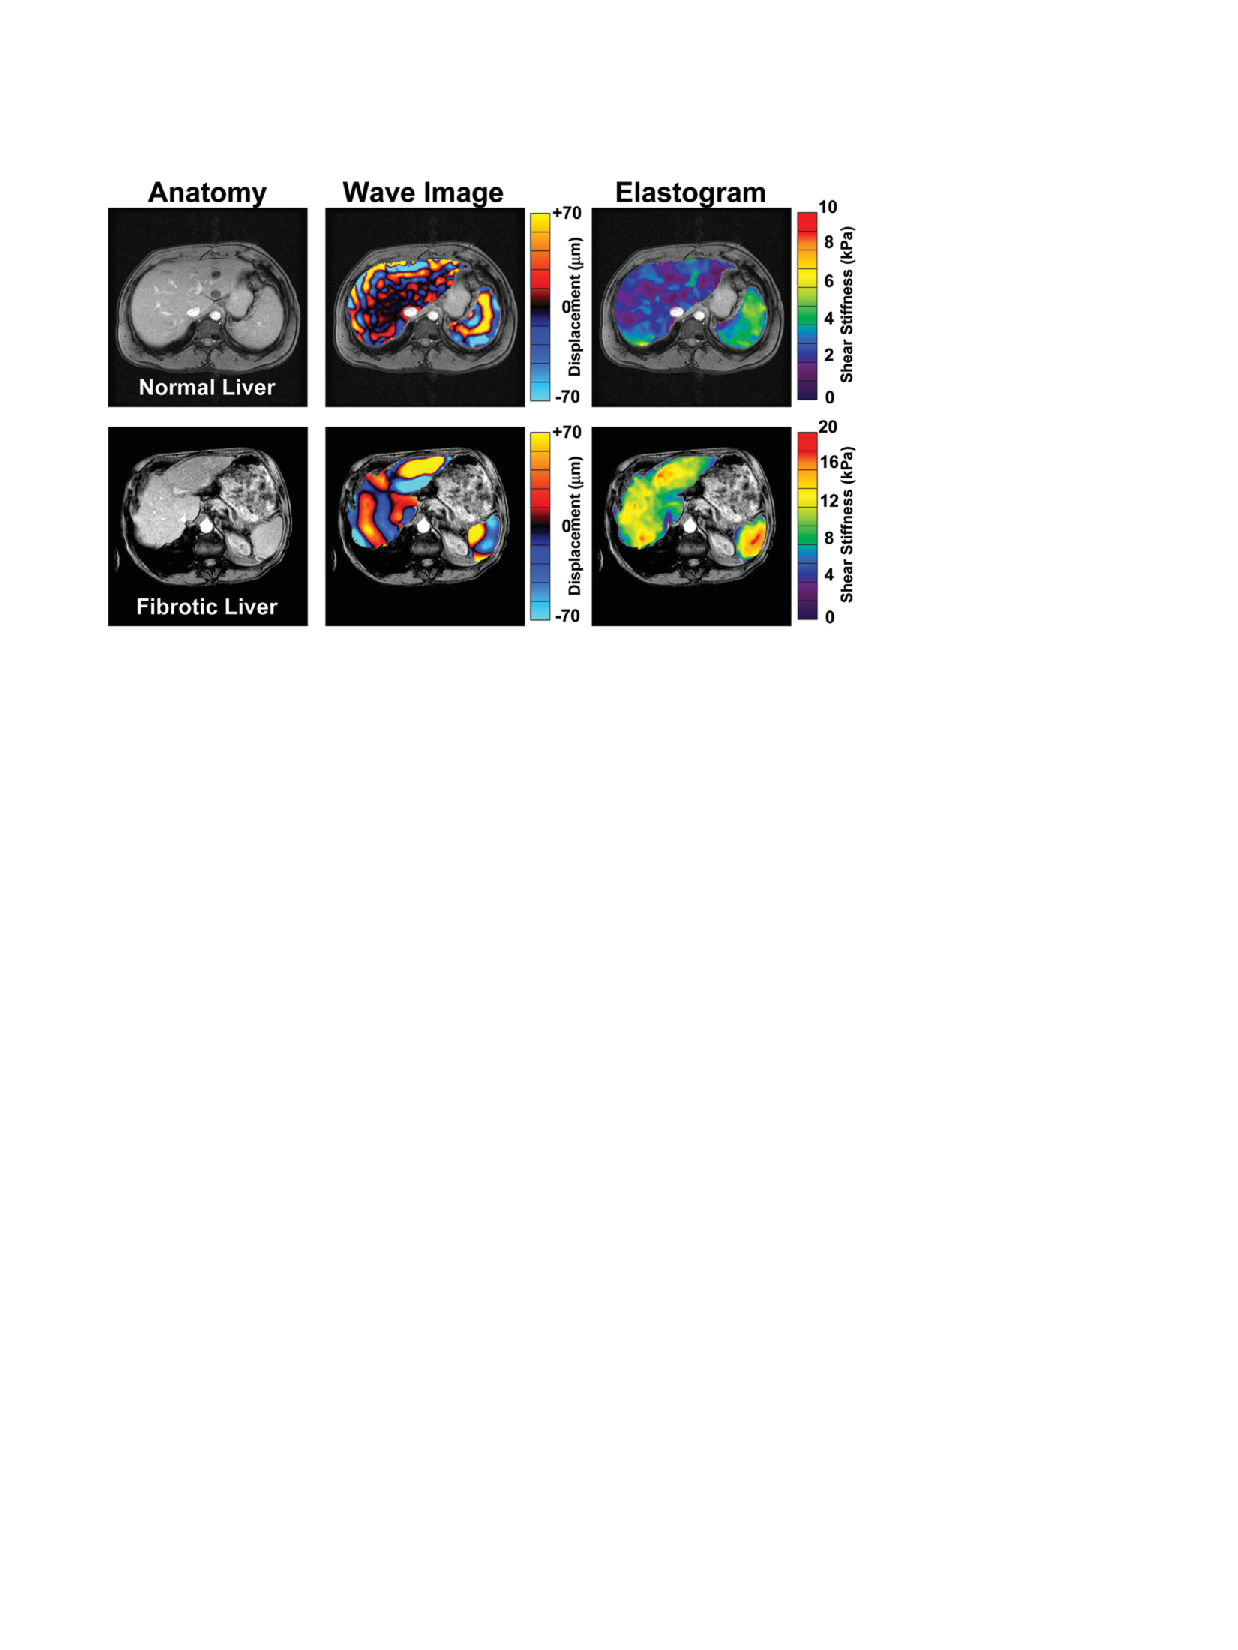
\includegraphics[width=12cm]{chapter2/elastography_liver.pdf}
\caption {\ON Magnetic resonance elastography of the liver in a healthy volunteer and a patient with cirrhosis. Image courtesy of \cite{Talwalkar07}.}
\label{chap2:fig-elastography_liver}
\end{figure}

Yet, precised characterisation of soft tissue is not sufficient to achieve a good simulation. The development of a simplified or optimised version of the model suitable for real-time computation is also mandatory. \OFF As we will see in chapter \ref{chap4} and \ref{chap7}, numerous models are available in the literature to describe physics of objects, from fairly simple and naive approaches to more complex and thorough representations. However, the most common technique to solve equations of continuum mechanics is the finite element method. Moreover, since the two main contributions of this thesis deal with finite element methods formulations, the general principles of this method will be detailed in the next section. 
